\documentclass[11pt,a4paper]{report}

\usepackage[utf8]{inputenc}
\usepackage[T1]{fontenc}
\usepackage[french]{babel}
\usepackage{lmodern}
\usepackage{geometry}
\usepackage{xcolor}
\usepackage{graphicx}
\usepackage{booktabs}
\usepackage{multirow}
\usepackage{array}
\usepackage{longtable}
\usepackage{tabularx}
\usepackage{listings}
\usepackage{fancyhdr}
\usepackage{titlesec}
\usepackage{hyperref}
\usepackage{enumitem}
\usepackage{float}
\usepackage{caption}
\usepackage{microtype}
\usepackage{tikz}
\usetikzlibrary{arrows.meta, positioning}

\geometry{top=2.2cm,bottom=2.2cm,left=2.4cm,right=2.4cm}
\definecolor{cmrpiblue}{RGB}{20,67,107}
\definecolor{cmrpilight}{RGB}{232,241,247}
\definecolor{codegreen}{RGB}{20,110,70}
\hypersetup{
  colorlinks=true,
  linkcolor=cmrpiblue,
  urlcolor=cmrpiblue,
  pdftitle={Rapport du Jalon 3 - MVP de détection et d'alerte},
  pdfauthor={ALLADO Kossi Richard et ADJEVI Kodjo Marius-Ben}
}

\pagestyle{fancy}
\fancyhf{}
\fancyhead[L]{Jalon 3 -- Projet de stage PFA}
\fancyhead[R]{CyberVeille PME}
\fancyfoot[L]{ALLADO Kossi Richard -- ADJEVI Kodjo Marius-Ben}
\fancyfoot[R]{Page \thepage}
\renewcommand{\headrulewidth}{0.4pt}
\renewcommand{\footrulewidth}{0.4pt}

\titleformat{\chapter}[hang]
  {\normalfont\huge\bfseries\color{cmrpiblue}}
  {\thechapter.}{0.7em}{}
\titlespacing*{\chapter}{0pt}{-20pt}{18pt}
\titleformat{\section}
  {\normalfont\Large\bfseries\color{cmrpiblue}}
  {\thesection}{0.7em}{}

\lstset{
  language=Python,
  basicstyle=\ttfamily\small,
  keywordstyle=\color{cmrpiblue}\bfseries,
  commentstyle=\color{codegreen},
  stringstyle=\color{purple},
  numbers=left,
  numberstyle=\tiny,
  stepnumber=1,
  numbersep=8pt,
  showstringspaces=false,
  breaklines=true,
  frame=single,
  backgroundcolor=\color{cmrpilight},
  captionpos=b
}

\newcommand{\metric}[2]{%
  \begin{minipage}[t]{0.22\textwidth}
    \centering
    \colorbox{cmrpilight}{\parbox[c][1.6cm][c]{0.92\linewidth}{%
      \centering\Large\bfseries\color{cmrpiblue}#1\\[-1mm]
      \normalsize\color{black}#2}}
  \end{minipage}
}

\begin{document}

\begin{titlepage}
  \centering
  {\large\bfseries Centre Marocain de Recherches Polytechnique et d'Innovation\par}
  \vspace{0.25cm}
  {\large Département / Service : Cybersécurité IA\par}
  \vspace{1.3cm}
  \rule{\textwidth}{1.2pt}
  \vspace{0.5cm}

  {\Large\bfseries PROJET DE STAGE PFA -- ÉTÉ 2026\par}
  \vspace{0.5cm}
  {\LARGE\bfseries\color{cmrpiblue}
  Système de détection et d'alerte précoce\\
  des cybermenaces ciblant les PME\par}

  \vspace{0.5cm}
  \rule{\textwidth}{1.2pt}
  \vspace{1.3cm}

  {\Large\bfseries LIVRABLE DU TROISIÈME JALON\par}
  \vspace{0.7cm}
  {\LARGE\bfseries
  Intégration du détecteur dans un MVP\\
  de veille, d'alerte et de réponse PME\par}
  \vspace{0.4cm}
  {\large Streamlit, Threat Intelligence, SQLite et SMTP\par}

  \vfill

  \begin{tabularx}{\textwidth}{X X}
    \textbf{Réalisé par :} & \textbf{Encadré par :}\\[0.25cm]
    ALLADO Kossi Richard & Pr. Youssef Bentaleb\\
    ADJEVI Kodjo Marius-Ben & Co-encadrante : Pr. Mehdia Ajana
  \end{tabularx}

  \vfill
  {\large\bfseries Période du troisième jalon\par}
  {\large Août 2026\par}
  \vspace{0.7cm}
  {\large Année universitaire 2025--2026\par}
\end{titlepage}

\pagenumbering{roman}
\tableofcontents
\clearpage
\pagenumbering{arabic}

\chapter{Introduction}

Le projet de stage PFA a pour objectif de proposer un prototype léger de
detection et d'alerte précoce face aux cybermenaces visant les petites et
moyennes entreprises (PME). Le cas d'usage retenu est le phishing par URL :
un employé reçoit un lien douteux, le transmet au système sans l'ouvrir, puis
reçoit une aide à la décision et, si nécessaire, une alerte est envoyée au
responsable concerné.

Le Jalon 2 a permis de réaliser le socle de détection. Un jeu de données
étiqueté PhiUSIIL a été préparé, 21 caractéristiques structurelles d'URL ont
été extraites et une régression logistique a été entraînée puis évaluée. Le
modèle sauvegardé a obtenu une accuracy de 99,32\,\% sur un jeu de test
indépendant. La collecte URLhaus a également été rendue incrémentale et
reproductible.

Le Jalon 3 transforme ce socle technique en un produit minimum viable (MVP)
utilisable par une PME. Les travaux portent sur l'intégration du modèle dans
une interface Streamlit, le croisement avec la Threat Intelligence URLhaus,
la conservation des analyses dans SQLite, l'envoi d'alertes par e-mail et la
mise à disposition de fiches réflexes. Ce rapport présente les objectifs
atteints, l'architecture, les tests fonctionnels et les résultats obtenus.

\chapter{Bilan du passage du Jalon 2 au Jalon 3}

\section{Acquis du Jalon 2}

Le Jalon 2 a fourni les composants analytiques réutilisés par le MVP :

\begin{itemize}
  \item un jeu de 235\,795 URL préparées, dont 100\,945 URL de phishing et
        134\,850 URL légitimes ;
  \item 21 caractéristiques lexicales et structurelles extraites localement ;
  \item une séparation entraînement/test stratifiée de 80\,\% / 20\,\% ;
  \item une régression logistique et un \texttt{StandardScaler} sauvegardés
        dans le dossier \texttt{models/} ;
  \item une base locale URLhaus mise à jour par le script
        \texttt{Download\_urls.py}.
\end{itemize}

Le modèle demeure volontairement simple et explicable. Le Jalon 3 ne le
réentraîne pas : il le charge et applique les mêmes transformations qu'à
l'entraînement. Cette décision garantit la cohérence entre les résultats
évalués au Jalon 2 et les prédictions affichées à l'utilisateur.

\section{Objectifs du Jalon 3}

Les objectifs fixés pour cette étape étaient les suivants :

\begin{enumerate}
  \item intégrer la détection d'URL dans une interface accessible ;
  \item enrichir la décision par une source de Threat Intelligence ;
  \item enregistrer l'historique des analyses ;
  \item envoyer une alerte e-mail pour les menaces prioritaires ;
  \item proposer des consignes de réaction adaptées aux PME ;
  \item valider le fonctionnement par des tests automatisés et manuels.
\end{enumerate}

\section{Résultats d'avancement}

\begin{table}[H]
\centering
\caption{Objectifs du Jalon 3 et état de réalisation}
\begin{tabularx}{\textwidth}{p{0.49\textwidth}cX}
\toprule
\textbf{Objectif} & \textbf{État} & \textbf{Réalisation}\\
\midrule
Interface de détection & Réalisé & Application Streamlit avec navigation et affichage des résultats.\\
Décision centralisée & Réalisé & Service combinant modèle ML et index local URLhaus.\\
Historique local & Réalisé & Base SQLite créée automatiquement.\\
Alertes e-mail & Réalisé & SMTP configurable, TLS/SSL et protection anti-doublon.\\
Analyse de masse & Réalisé & Import CSV, traitement de 1\,000 URL au maximum et export des résultats.\\
Fiches réflexes & Réalisé & Trois fiches : lien suspect, clic et identifiants compromis.\\
Réputation IP & Optionnel & Extension AbuseIPDB disponible si une clé est configurée.\\
\bottomrule
\end{tabularx}
\end{table}

\chapter{Architecture du MVP}

\section{Vue d'ensemble}

Le MVP est organisé autour de l'application \texttt{app.py}. Cette interface
appelle un service central, qui effectue une analyse statique : aucune URL
n'est ouverte et aucune page distante n'est chargée. L'architecture sépare la
présentation, la décision, la persistance et la notification.

\begin{center}
\begin{tikzpicture}[
  node distance=1.3cm and 2cm,
  every node/.style={font=\normalsize, align=center},
  ->, >=Stealth
]

% Top row
\node (pme) {Employé PME};
\node (app) [right=of pme] {Streamlit (\texttt{app.py})};
\node (detect) [right=of app] {service de détection};

\draw (pme) -- (app);
\draw (app) -- (detect);

% Middle row: build outward from the center node, not from the top row
\node (ml) [below=1.3cm of app, text width=3.2cm] {Caractéristiques + modèle ML};
\node (urlhaus) [left=2.2cm of ml] {URLhaus local};
\node (sqlite) [right=2.2cm of ml] {SQLite / SMTP};

\draw (app) -- (ml);
\draw (app) -- (urlhaus);
\draw (app) -- (sqlite);
% Bottom row
\node (decision) [below=1.3cm of ml, text width=8cm] {Décision, recommandations et éventuelle alerte};

\draw (ml) -- (decision);
\draw (urlhaus) -- (decision);
\draw (sqlite) -- (decision);
\end{tikzpicture}
\end{center}
\section{Composants développés}

\begin{longtable}{p{0.31\textwidth}p{0.59\textwidth}}
\caption{Principaux composants du Jalon 3}\\
\toprule
\textbf{Fichier ou dossier} & \textbf{Rôle}\\
\midrule
\endfirsthead
\toprule
\textbf{Fichier ou dossier} & \textbf{Rôle}\\
\midrule
\endhead
\texttt{app.py} & Interface Streamlit : tableau de bord, analyse unitaire,
analyse CSV, historique, alertes, fiches réflexes et configuration.\\
\texttt{detection\_service.py} & Validation, chargement du modèle, recherche
URLhaus, calcul du risque, explications et recommandations.\\
\texttt{database.py} & Création et accès à la base SQLite des analyses et
des états d'alerte.\\
\texttt{alert\_service.py} & Lecture de la configuration, construction de
l'e-mail, envoi SMTP et anti-doublon.\\
\texttt{ip\_reputation\_service.py} & Interrogation facultative d'AbuseIPDB
pour une adresse IP, seulement lorsqu'une clé est présente.\\
\texttt{fiches\_reflexes/} & Procédures courtes destinées à l'utilisateur
après la détection d'un lien, d'un clic ou d'identifiants saisis.\\
\texttt{tests/test\_mvp.py} & Tests automatisés du pipeline métier.\\
\bottomrule
\end{longtable}

\section{Parcours d'une analyse}

Lorsqu'une URL est saisie, le système suit les étapes suivantes :

\begin{enumerate}
  \item validation du format HTTP ou HTTPS et normalisation de l'URL ;
  \item recherche de l'URL dans le fichier local
        \texttt{data/collected/urlhaus/current\_urls.csv} ;
  \item extraction des 21 caractéristiques avec
        \texttt{feature\_engineering.py} ;
  \item standardisation avec le scaler du Jalon 2 et prédiction par la
        régression logistique ;
  \item attribution d'un niveau de risque et génération d'explications ;
  \item enregistrement de l'analyse dans SQLite ;
  \item envoi d'une alerte si le seuil configuré est atteint.
\end{enumerate}

\section{Règles de décision}

La source URLhaus et le modèle ont des rôles complémentaires. URLhaus permet
de reconnaître une menace déjà connue dans la base locale. Le modèle estime le
risque pour une URL inconnue à partir de sa forme. L'absence de correspondance
URLhaus ne signifie donc pas qu'une URL est sûre.

\begin{table}[H]
\centering
\caption{Niveaux de risque appliqués par le service de détection}
\begin{tabular}{ll}
\toprule
\textbf{Niveau} & \textbf{Règle}\\
\midrule
Critique & Correspondance exacte dans la base URLhaus locale.\\
Élevé & Probabilité de phishing supérieure ou égale à 85\,\%.\\
Moyen & Probabilité de phishing comprise entre 55\,\% et 85\,\%.\\
Faible & Probabilité de phishing inférieure à 55\,\%.\\
\bottomrule
\end{tabular}
\end{table}

Les résultats comportent également des raisons compréhensibles : utilisation
d'une adresse IP comme hôte, absence de HTTPS, présence de mots-clés suspects,
nombre important de sous-domaines ou longueur inhabituelle de l'URL.

\chapter{Fonctionnalités livrées}

\section{Interface Streamlit}

L'application est lancée avec la commande suivante :

\begin{lstlisting}[language={},caption={Lancement du MVP}]
streamlit run app.py
\end{lstlisting}

Sept pages sont disponibles :

\begin{itemize}
  \item \textbf{Tableau de bord} : nombre d'analyses, menaces et alertes,
        ainsi que les analyses récentes ;
  \item \textbf{Analyser une URL} : saisie d'un indicateur URL et consultation
        du résultat ;
  \item \textbf{Analyse en masse} : import d'un CSV contenant une colonne
        \texttt{url}, avec téléchargement du résultat ;
  \item \textbf{Historique} : consultation et filtrage des analyses SQLite ;
  \item \textbf{Alertes} : état de la configuration SMTP sans divulgation
        des secrets ;
  \item \textbf{Fiches réflexes} : actions prioritaires pour l'utilisateur ;
  \item \textbf{Configuration} : exemple des variables nécessaires et
        limites du prototype.
\end{itemize}

\section{Historique SQLite}

La base locale \texttt{data/threats.db} est créée automatiquement. Elle
enregistre l'URL analysée, la date, le verdict du modèle, la probabilité, le
niveau de risque, le résultat URLhaus, les explications et l'état de l'envoi
d'alerte. Les requêtes SQL utilisent des paramètres et les connexions sont
fermées systématiquement. Cette base est exclue du dépôt Git afin de ne pas
publier les données opérationnelles d'une PME.

\section{Alertes SMTP}

Les paramètres de messagerie sont lus depuis le fichier local \texttt{.env},
qui est également exclu de Git. Aucun mot de passe n'est présent dans le code
ou dans le rapport. Le service prend en charge STARTTLS, SSL ou une connexion
SMTP non chiffrée lorsque cela est explicitement configuré. Pour le test, un
compte Gmail a utilisé SMTP avec STARTTLS et un mot de passe d'application.

Avant l'envoi, le système vérifie que le niveau de risque atteint le seuil
\texttt{ALERT\_MIN\_RISK}. Il vérifie aussi qu'une alerte réussie pour la même
URL n'a pas déjà été transmise dans la fenêtre
\texttt{ALERT\_DEDUP\_MINUTES}. Une erreur SMTP est affichée et historisée,
mais elle ne supprime pas l'analyse.

\section{Fiches réflexes}

Trois fiches pratiques complètent la détection technique :

\begin{enumerate}
  \item \textbf{Lien suspect reçu} : ne pas cliquer, vérifier l'expéditeur
        et signaler le message ;
  \item \textbf{L'utilisateur a cliqué} : isoler si nécessaire, fermer la
        page, prévenir le responsable et surveiller le poste ;
  \item \textbf{Identifiants saisis} : changer les mots de passe, révoquer les
        sessions et avertir rapidement l'équipe informatique.
\end{enumerate}

\chapter{Tests et résultats}

\section{Tests automatisés}

Le fichier \texttt{tests/test\_mvp.py} contient 12 tests exécutés avec :

\begin{lstlisting}[language={},caption={Exécution des tests}]
python -m unittest discover -s tests -v
\end{lstlisting}

Les 12 tests ont été exécutés avec succès. Ils couvrent les entrées vides ou
invalides, l'ajout automatique d'un protocole, une URL légitime, une URL
suspecte avec une adresse IP, la présence et l'absence dans URLhaus, une
analyse de liste, l'absence d'artefact ML, l'indisponibilité d'URLhaus, la
persistance SQLite, les alertes désactivées et l'échec SMTP.

\begin{center}
\metric{12 / 12}{Tests réussis}\hfill
\metric{0}{Échec de test}\hfill
\metric{99,32\,\%}{Accuracy Jalon 2}\hfill
\metric{2}{Tests manuels présentés}
\end{center}

\vspace{0.6cm}

La couverture automatisée confirme notamment que l'application échoue de
façon contrôlée lorsqu'une dépendance locale est indisponible et que l'échec
d'envoi d'un e-mail ne bloque pas l'enregistrement du résultat.

\section{Test fonctionnel d'une URL légitime}

Le premier scénario vérifie qu'une URL largement utilisée et sans indicateur
lexical notable ne produit pas une alerte injustifiée. L'URL
\url{https://www.google.com} a été analysée dans l'interface.

\begin{figure}[H]
  \centering
  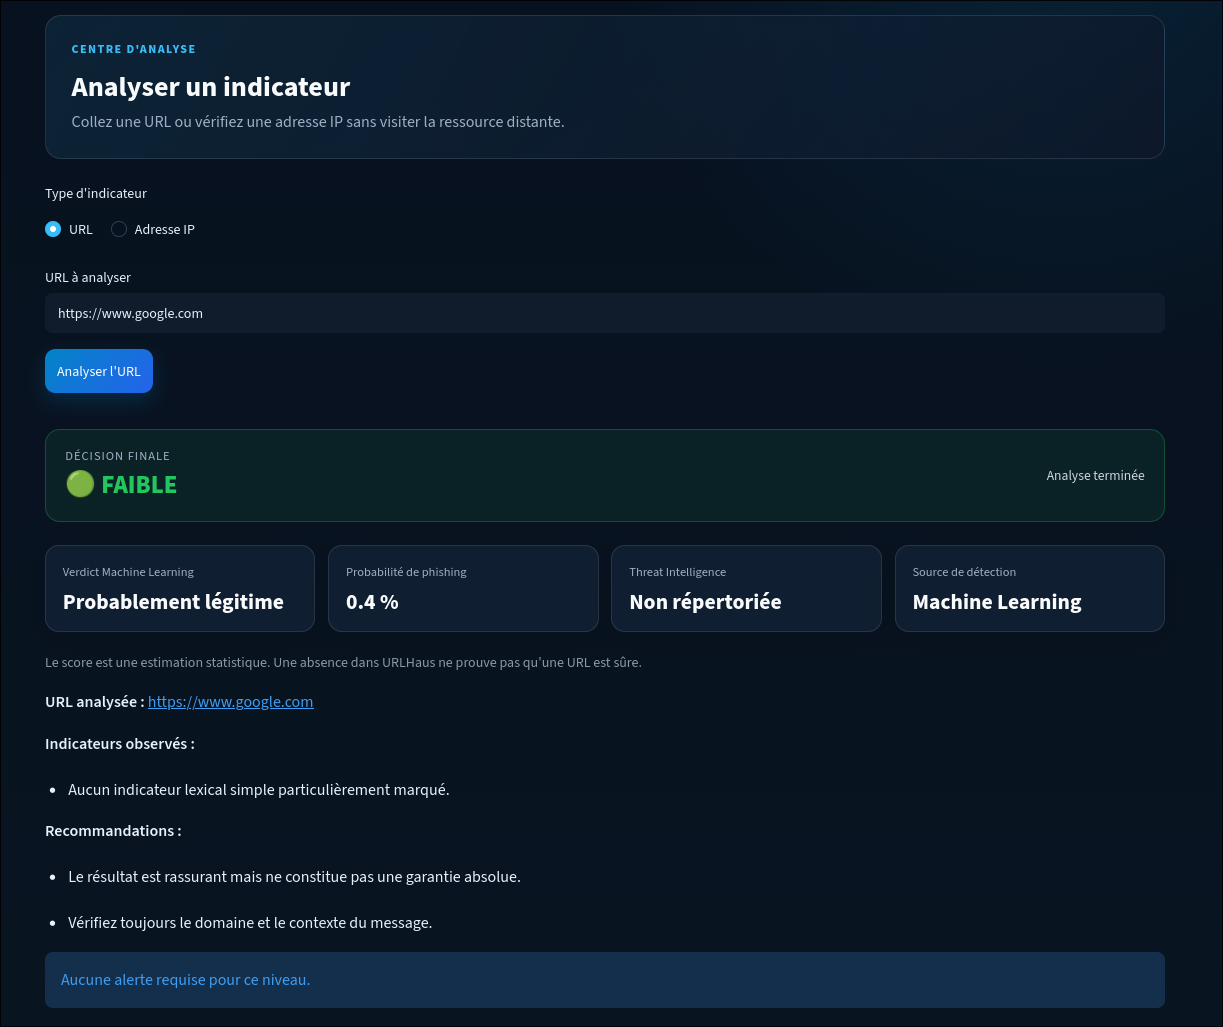
\includegraphics[width=0.7\textwidth]{img/test_for_legitime_google_url.png}
  \caption{Résultat du test fonctionnel avec l'URL légitime Google}
  \label{fig:google-test}
\end{figure}

La figure~\ref{fig:google-test} montre un risque \textbf{Faible}, un verdict
\og Probablement légitime \fg{} et une probabilité de phishing de 0,4\,\%.
L'URL n'est pas répertoriée dans URLhaus et aucune alerte n'est requise. Ce
test illustre le comportement attendu pour limiter les faux positifs dans un
cas d'usage courant.

\section{Test fonctionnel d'une URL suspecte sûre pour la démonstration}

Le second scénario utilise l'URL suivante :

\begin{center}
\url{http://192.0.2.10/secure-login/verify-account?password=confirm\&case=1}
\end{center}

L'adresse \texttt{192.0.2.10} appartient à une plage réservée à la
documentation ; elle n'est pas utilisée comme un site réel. Le test est donc
réalisé sans ouvrir ni consulter une ressource distante. L'URL contient
cependant plusieurs signaux volontairement suspects : une adresse IP comme
hôte, l'absence de HTTPS et les mots-clés \texttt{secure}, \texttt{login},
\texttt{verify}, \texttt{account}, \texttt{password} et \texttt{confirm}.

\begin{figure}[H]
  \centering
  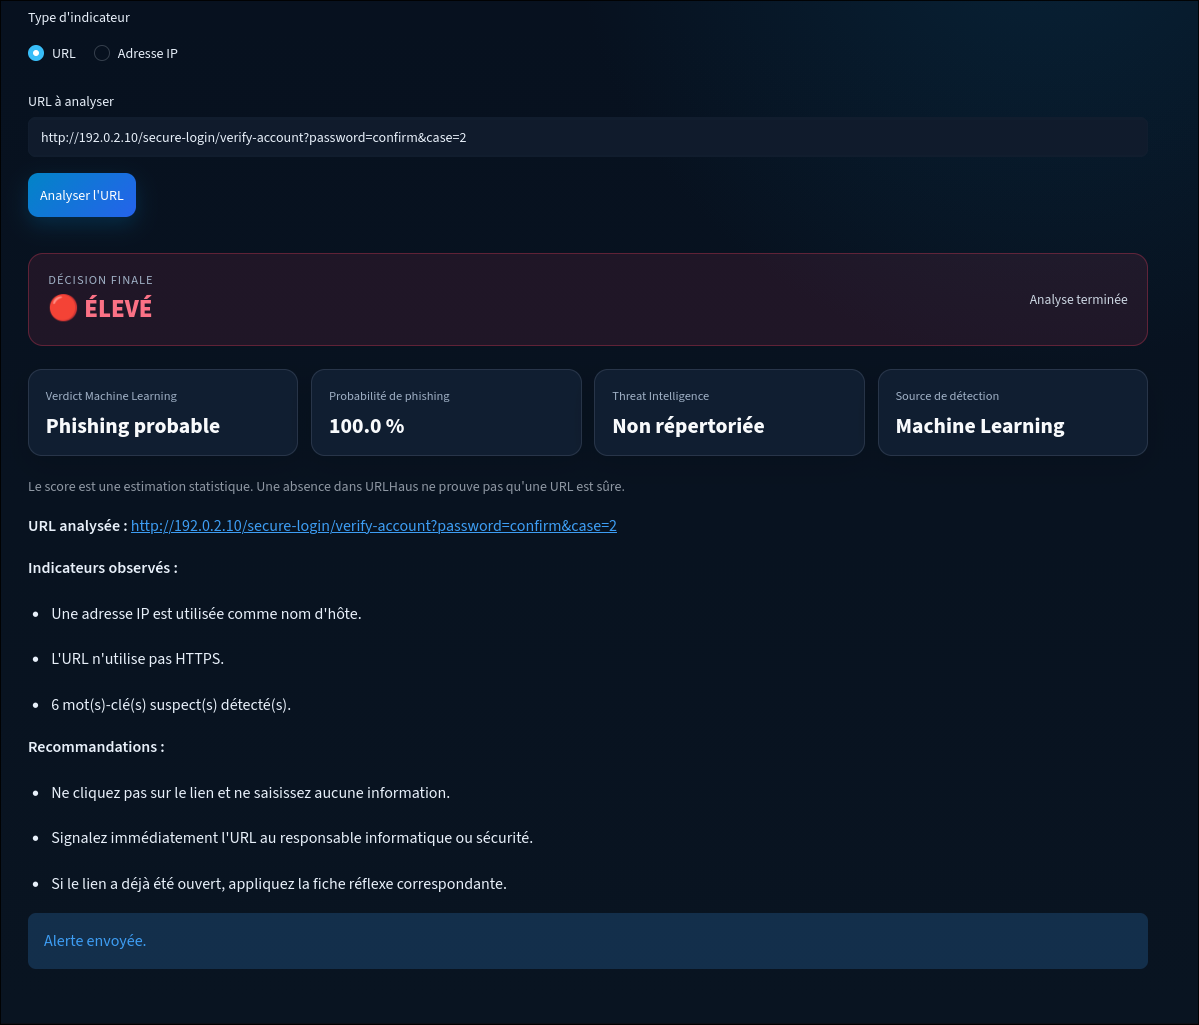
\includegraphics[width=0.92\textwidth]{img/test_for_bad_url.png}
  \caption{Détection d'une URL de démonstration à risque élevé}
  \label{fig:suspicious-test}
\end{figure}

Le système retourne le verdict \og Phishing probable \fg{}, une probabilité de
phishing de 100,0\,\% et le niveau \textbf{Élevé}. Il affiche les trois
raisons attendues : adresse IP, absence de HTTPS et six mots-clés suspects.
La capture montre également le message d'anti-doublon ; celui-ci est normal
lorsqu'une alerte pour cette même URL a déjà été envoyée récemment.

\section{Test d'envoi d'une alerte réelle}

La configuration SMTP a ensuite été activée dans le fichier local
\texttt{.env}. Le même compte Gmail a servi d'expéditeur et de destinataire
pour la démonstration. Cette configuration est adaptée à un test isolé ; dans
une PME, le destinataire doit être l'adresse du responsable informatique ou
sécurité.

\begin{figure}[H]
  \centering
  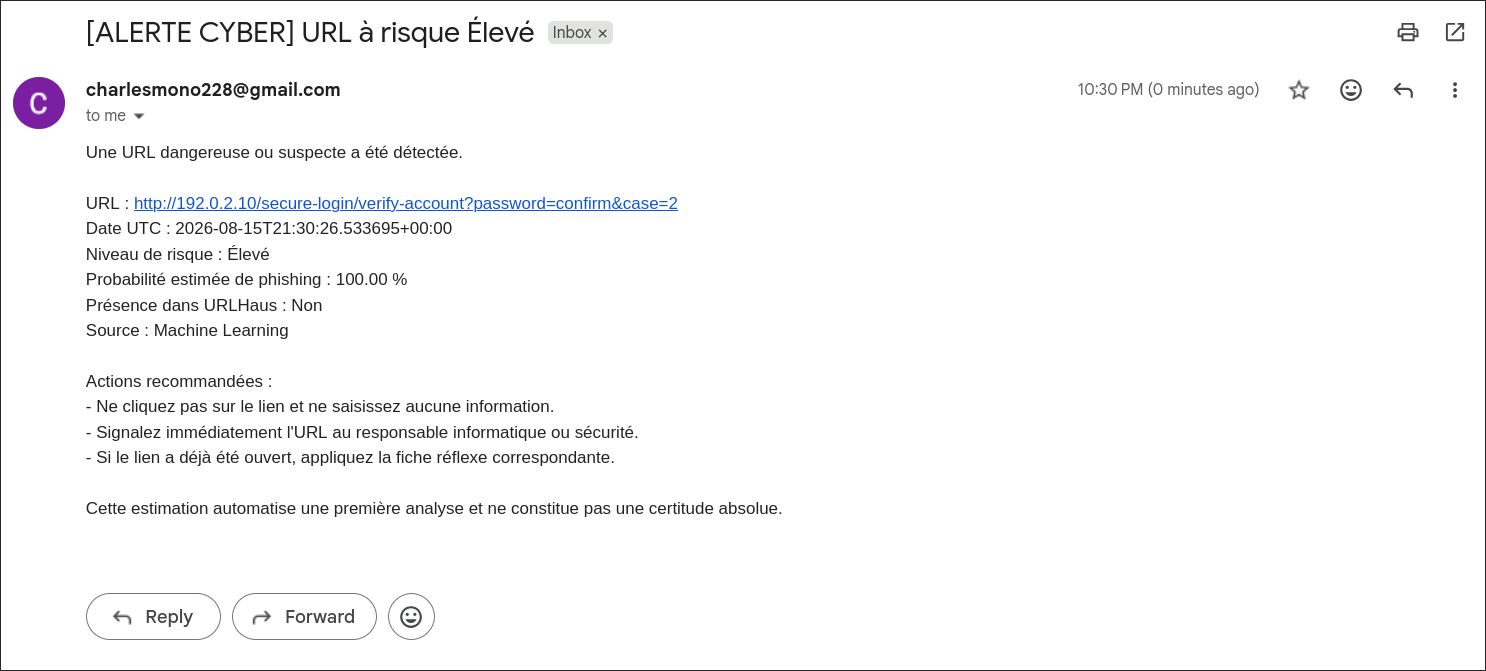
\includegraphics[width=\textwidth]{img/Alert_received.png}
  \caption{E-mail d'alerte reçu après la détection de l'URL à risque élevé}
  \label{fig:alert-test}
\end{figure}

Comme le montre la figure~\ref{fig:alert-test}, l'e-mail porte le sujet
\og [ALERTE CYBER] URL à risque Élevé \fg{}. Son contenu reprend l'URL
analysée, la date UTC, le niveau de risque, la probabilité estimée, le statut
URLhaus, la source de détection et les actions recommandées. L'envoi réel
confirme le fonctionnement de bout en bout du mécanisme d'alerte.

\begin{table}[H]
\centering
\caption{Synthèse des tests fonctionnels manuels}
\begin{tabularx}{\textwidth}{p{0.28\textwidth}p{0.24\textwidth}p{0.20\textwidth}X}
\toprule
\textbf{Scénario} & \textbf{Résultat observé} & \textbf{Alerte} & \textbf{Conclusion}\\
\midrule
\url{https://www.google.com} & Faible ; 0,4\,\% ; probablement légitime & Non & Comportement rassurant, sans faux positif visible.\\
URL de démonstration avec IP et mots-clés & Élevé ; 100,0\,\% ; phishing probable & Oui & Détection des indices lexicaux et déclenchement de l'alerte.\\
Réexécution de la même URL & Résultat conservé & Non, si récent & Protection anti-doublon opérationnelle.\\
\bottomrule
\end{tabularx}
\end{table}

\chapter{Sécurité, limites et perspectives}

\section{Mesures de sécurité appliquées}

Le prototype adopte les précautions suivantes :

\begin{itemize}
  \item les URL sont analysées comme des chaînes de caractères et ne sont pas
        ouvertes par l'application ;
  \item seules les URL HTTP et HTTPS correctement formées sont acceptées ;
  \item les secrets SMTP et la clé AbuseIPDB restent dans \texttt{.env}, hors
        du dépôt Git ;
  \item la base SQLite d'incidents est également exclue de Git ;
  \item les connexions SMTP utilisent STARTTLS ou SSL selon la configuration ;
  \item l'anti-doublon limite les notifications répétitives ;
  \item une indisponibilité de service ne doit pas interrompre l'analyse.
\end{itemize}

\section{Limites}

Le résultat reste une aide à la décision et non une preuve absolue de
malveillance ou de légitimité. Le modèle n'analyse ni le contenu de la page,
ni les redirections, ni les pièces jointes, ni la réputation complète du
domaine. Une URL inconnue d'URLhaus peut être dangereuse, et une URL
légitime peut contenir des termes semblant suspects.

Les performances élevées mesurées au Jalon 2 sont liées au jeu de test
PhiUSIIL. Elles doivent être suivies lorsque de nouvelles sources de données
ou de nouveaux types d'attaques sont intégrés. Enfin, l'extension AbuseIPDB
reste facultative et dépend d'une clé API ainsi que de la disponibilité du
service distant.

\section{Perspectives}

Les améliorations envisagées après la validation du MVP sont :

\begin{enumerate}
  \item tester régulièrement l'interface sur un poste de démonstration et
        documenter les cas limites ;
  \item planifier automatiquement la mise à jour URLhaus ;
  \item enrichir le rapport final avec des captures supplémentaires et une
        démonstration vidéo de secours ;
  \item étudier un déploiement Streamlit adapté à une PME ;
  \item étudier l'intégration encadrée de boîtes Gmail ou Outlook, avec
        consentement et analyse de confidentialité ;
  \item compléter éventuellement la réputation IP par AbuseIPDB.
\end{enumerate}

\chapter{Conclusion}

Le Jalon 3 a permis de faire évoluer le détecteur développé au Jalon 2 vers
un MVP opérationnel destiné aux PME. La régression logistique et les 21
caractéristiques existantes sont désormais exploitées dans une interface
Streamlit. La décision combine le score du modèle avec une recherche dans la
base locale URLhaus, puis fournit un niveau de risque, des explications et des
recommandations pratiques.

Les objectifs essentiels sont atteints : analyse unitaire et en masse,
historique SQLite, alertes SMTP, fiches réflexes et extension IP facultative.
Les 12 tests automatisés sont réussis. Les tests manuels montrent qu'une URL
légitime est classée à risque faible, tandis qu'une URL de démonstration
présentant des indices suspects est classée à risque élevé et déclenche un
e-mail reçu avec succès.

Le prototype constitue ainsi une base cohérente pour la démonstration finale.
Ses limites sont explicitement prises en compte : il ne visite pas les URL,
ne remplace pas une analyse humaine et doit être enrichi progressivement
avant un éventuel déploiement opérationnel.

\chapter*{Références}
\addcontentsline{toc}{chapter}{Références}

\begin{itemize}
  \item URLhaus, abuse.ch : \url{https://urlhaus.abuse.ch}
  \item Documentation Streamlit : \url{https://docs.streamlit.io}
  \item Documentation Python \texttt{smtplib} :
        \url{https://docs.python.org/3/library/smtplib.html}
  \item Documentation SQLite : \url{https://www.sqlite.org/docs.html}
  \item Documentation scikit-learn : \url{https://scikit-learn.org/stable/}
  \item PhiUSIIL Phishing URL Dataset, UCI Machine Learning Repository :
        \url{https://archive.ics.uci.edu/dataset/967/phiusiil+phishing+url+dataset}
  \item Dépôt GitHub du projet :
        \url{https://github.com/ALLAKORI/STAGE_PFA_CMRPI}
\end{itemize}

\appendix
\chapter{Reproduction du MVP}

\begin{lstlisting}[language={},caption={Installation et lancement}]
python -m venv venv
source venv/bin/activate
pip install -r requirements.txt
streamlit run app.py
\end{lstlisting}

Pour activer les alertes, l'utilisateur copie \texttt{.env.example} vers
\texttt{.env}, renseigne les paramètres SMTP et laisse ce fichier hors du
dépôt. Les tests sont rejoués avec :

\begin{lstlisting}[language={},caption={Commande de validation}]
python -m unittest discover -s tests -v
\end{lstlisting}

\end{document}
\documentclass{article}
\usepackage{graphicx} % Required for inserting images

\title{Stage_C}
\author{Kodjo Marius-Ben ADJEVI}
\date{August 2026}

\begin{document}

\maketitle

\section{Introduction}

\end{document}
